\chapter{Methodology}\label{chap:key:4}
\section{The ``Language Situations'' method }\label{sec:key:4.1}

The method used for data collection for this study is called ``Language Situations'', developed by \citet{Wiese2020} and later refined by members of the ‘Research Unit Emerging Grammars’ (RUEG). This method was developed to capture actual language use while simultaneously maintaining sufficient control over participants' productions to gather comparable data relevant to specific research questions. In doing so, it combines the benefits of controlled elicitation with those of natural data collection. Furthermore, it captures language productions across different communicative situations, allowing comparisons across informal and formal settings and spoken and written modes.

\largerpage
The stimulus is a short (one-minute) video clip depicting a staged car accident. After watching it, participants were asked to imagine that they had witnessed this accident. Their task was to describe what they had seen in four different communicative situations: to their close friend via a WhatsApp voice message (informal spoken) and a WhatsApp text message (informal written), to report the accident to the police via a voice recorder (formal spoken) and to write a witness report to the police (formal written). These situations were labelled as formal and informal for the purposes of the study. At the same time, formal and informal communication should not be understood as fixed or homogeneous categories, as they can be realized in a range of different communicative situations. In the present design, situational variation was therefore operationalized specifically through the addressee, the medium of communication, and the spoken versus written mode. For ease of reference, the labels formal spoken, formal written, informal spoken, and informal written are used throughout the manuscript.

\begin{figure}
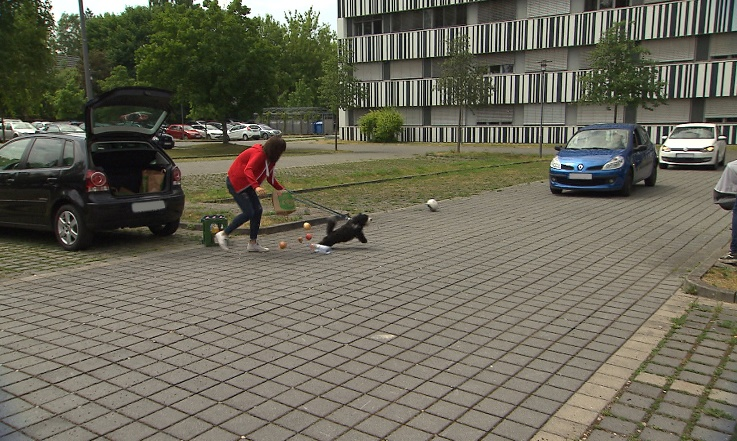
\includegraphics[width=\textwidth]{figures/iefremenko-img005.jpg}
\caption{\label{fig:key:4.1}A screenshot from the video stimulus.}
\end{figure}

There was a break of approximately 10--15 minutes between the informal and formal elicitations. Bilingual participants completed the task in both languages, heritage and majority\footnote{As shown in Section 2.3, Kurmanji speakers have been reported to experience language anxiety when using Turkish, primarily based on adolescent populations (see \citealt{Sahin-firat2010}). In the present study, however, which includes adult participants, no overt anxiety or resistance to speaking Turkish was observed. All participants lived in Ankara and used Turkish in their daily lives.}, while trilingual speakers in Germany did it in their heritage languages, Kurmanji and Turkish.\footnote{German was not collected for the trilingual participants because the aim of the study was to focus specifically on the trilingual speakers’ heritage languages.} There was a break of at least three days, but typically a week, between the sessions. It is also important to note that in informal situations, the elicitor instructed participants to imagine that they were talking to a friend with whom they usually spoke in the tested language. To prevent potential priming effects, the order of the communicative situations and languages was balanced. Depending on the number of participants in each group, at least one, and in most cases two, participants were assigned to each order (heritage vs. majority, formal vs. informal, spoken vs. written). The table with the orders can be found here: https://osf.io/m82qe.

To obtain data that reflected natural language use in both informal and formal contexts, it was essential to create a realistic environment. As the experiment was conducted mostly in universities, schools, or offices, establishing a formal atmosphere was relatively straightforward. Typically, the setting consisted of a classroom furnished with a table and two chairs. The table held only a laptop, a voice recording device, and consent forms. A formally dressed elicitor conducted the session, interacting with participants using formal language, explaining the elicitation procedure, and requesting signatures on the consent forms. Creating a comfortable and relaxed informal setting proved more challenging. For this purpose, a smaller, well-lit room decorated with colorful rugs, flowers, and a tablecloth was chosen. Refreshments such as cookies, tea, and coffee were provided. A different elicitor, dressed casually, engaged participants in friendly conversation. Each participant first spent 12--15 minutes chatting with this informal elicitor about topics such as free time, hobbies, favorite music, books, and movies. These measures aimed to foster a welcoming atmosphere and help participants feel as comfortable and relaxed as possible.

Data collection took place between October 2018 and February 2020. All participants signed a written consent form that clarified data protection issues in accordance with the General Data Protection Regulation (GDPR) of the European Union. The study received approval from the ethics committee of the German Linguistics Society (\textit{Ethikkommission der Deutschen Gesellschaft für Sprachwissenschaft}). The entire elicitation process was recorded using a Tascam DR-05X voice recorder. A black Fujitsu laptop with a 15.6-inch screen was used to display videos and facilitate the writing of formal texts. For written productions, participants typed a WhatsApp text message using an iPhone 6 and a witness report on the laptop, where they could choose from various keyboards depending on the language. Participants in Germany had the option to use either a German keyboard or an external Turkish keyboard. Additionally, Kurmanji participants were informed where to find diacritics for some of the Kurmanji letters.

Collecting metalinguistic data from participants involved using a comprehensive questionnaire inspired by the one developed in the MULTILIT project \citep{SchroederEtAl2015} and further refined by the RUEG project team. The questionnaire consisted of ten sections, covering administration, general participant information, educational background, language proficiency, family background, self-assessment of language skills, language use with family members and peers, media consumption and leisure activities, personal character traits, and feedback on their participation in the study. It was available in both German and Turkish, allowing participants to complete it in the majority language of the country they reside in. Participants always filled out the questionnaire in the presence of an elicitor.

Several limitations should be considered when employing the 'Language Situations' method. Firstly, despite the natural context, many speakers may encounter situations, such as reporting an accident to the police, in their heritage language for the first time. For example, in Turkey, Kurmanji is not used in formal public settings, and interactions with governmental institutions typically occur in Turkish. However, even if participants lack experience in reporting accidents to the police in their heritage language, they are likely to possess knowledge of formal registers in the dominant language of their country, which is usually acquired through education. Therefore, one of the rationales for eliciting witness reports in participants’ heritage language is to capture their innovative strategies for using structures characteristic of formal language, drawing upon their understanding of language registers.

Furthermore, this method has limitations regarding the analysis of information structure. It was designed so that each speaker retold the accident four times across different communicative situations. Additionally, bilingual participants were asked to do the same in both of their languages, with a minimum break of three days between sessions. This means that bilingual participants narrated the same story a total of eight times, while monolingual participants retold it four times.

More information about the method, including consent forms, data collection instructions, questionnaires in PDF format, and elicitation orders, is publicly available in the Open Science Framework (OSF) repository at https://osf.io/qhupg/.

\section{Participants}\label{sec:key:4.2}

The study involved four groups of participants: heritage speakers of Turkish in Germany, heritage speakers of Kurmanji and Turkish in Germany, Kurmanji-Turkish bilinguals in Turkey, and Turkish monolinguals in Turkey. \tabref{tab:key:4.1} below presents information on the number of speakers in each group, as well as their age, gender, and languages.

\begin{table}\small
\begin{tabularx}{\textwidth}{l X c l c X X}
\lsptoprule
Country & Group & N & Mean age & Gender & Heritage language(s) & Majority language\\
\midrule
{Germany}
 & Turkish--German bilinguals & 33 & 27.14 & 23F & Turkish & German\\
\midrule
& Kurmanji-Turkish-German trilinguals & 9 & 24.34 & 8F & Kurmanji, Turkish & German\\
\midrule
{Turkey}
 & Kurmanji--Turkish bilinguals & 30 & 28.16 & 10F & Kurmanji & Turkish\\
\midrule
 & Turkish monolinguals & 32 & 27.63 & 11F & — & Turkish\\
\lspbottomrule
\end{tabularx}
\caption{\label{tab:key:4.1}Participant metadata.}
\end{table}

As indicated in \tabref{tab:key:4.1}, each group consists of approximately 30 speakers, with the exception of the trilingual group in Germany. The smaller number of speakers in this group is primarily due to a later start in data collection, which began in the Summer of 2019, and an abrupt halt in March 2020 caused by the pandemic outbreak and subsequent restrictions on in-person meetings. As will be discussed in the following chapters, the smaller size of the dataset from the trilingual speaker group leads to reliance on observations rather than statistical analyses. Consequently, this limitation poses challenges in making definitive statements regarding potential changes in word order within this speaker group.

The selection of participants for the study was guided by several criteria. The first criterion was age, as all participants were young adults between 25 and 35 years old. The second criterion focused on literacy, requiring participants to have reading and writing skills in the languages in which they were tested. Only speakers who had not attended bilingual schools were recruited, although some participants had received heritage language education, such as in Saturday schools. Additional criteria included the absence of speech or hearing disorders and residence in urban areas at the time of testing. Data from heritage speakers in Germany were collected in Berlin, Kurmanji-Turkish bilinguals were tested in Ankara, and Turkish monolinguals were assessed in İzmir and Eskişehir.

Additionally, participants needed to meet the definition of heritage speakers. For the heritage speakers of Turkish and Kurmanji in Germany, the age of arrival in Germany was a critical factor. Consequently, participants in the study were either born and raised in Germany or arrived in Germany before the age of two. Furthermore, they acquired their heritage language(s) in informal settings and used them with at least one family member. For Kurmanji speakers in Turkey, it was essential to ensure that they used the language at home and did not acquire it as a second language in a formal setting. Regarding monolingual speakers, a critical criterion was that they were raised exclusively in one language. Consequently, participants who used Kurmanji, Zazaki, Greek, or any other language within their family setting were excluded from the monolingual group. While some participants raised monolingually could speak additional foreign languages such as English, German, or Russian, they learned these as foreign languages.

Although participants were expected to meet specific criteria, there is considerable individual variation among the speakers concerning language dominance, proficiency, and attitudes, among other factors. For example, the trilingual group in Germany, which consists of speakers with two heritage languages, exhibits significant heterogeneity in the status of their languages. Some individuals favor Turkish within their families, with Kurmanji being understood but not actively taught to children, while others use exclusively Kurmanji at home but often speak Turkish in the neighborhood. Factors such as family dynamics and the surrounding environment contribute to this complexity. While the study will emphasize individual variation among speakers, it will not explore the potential factors behind this variation.

\section{The RUEG corpus}\label{sec:key:4.3}

To ensure anonymity, each file containing a participant’s production was assigned a unique code. The participant codes conveyed the following information: Country: DE for Germany and TU for Turkey, -lingualism: tr-, bi-, or monolingual speaker (tr, bi, or mo), speaker number: 1 to 49, gender: M for male and F for female (there were no speakers who identified as non-binary), heritage language for bilingual speakers or the majority language for monolinguals: T for Turkish and K for Kurmanji, formality: f for formal and i for informal, mode: s for spoken and w for written, and language of elicitation: T for Turkish and K for Kurmanji. For example, the code DEbi05MT\_isT indicates an informal spoken production in Turkish by a male bilingual speaker from Germany, whose heritage language is Turkish.

Following data collection, the recordings were transcribed using Praat software (\citealt{BoersmaWeenink2023}). After transcription, the data were normalized, segmented into communication units, and annotated for various linguistic phenomena using the Partitur-Editor component of the EXMARaLDA annotation software (\citealt{SchmidtWorner2014}). Normalization and annotation were conducted by native speakers of Turkish and Kurmanji. For Turkish normalization, the standards provided by the \textit{Türk Dil Kurumu} (Turkish Language Association) were used. In contrast, Kurmanji texts were normalized using the Kurmanji-English dictionary \citep{Chyet2003}. The data were segmented into communication units (CUs), defined as independent clauses along with their modifiers and dependent clauses, following \citet[9]{Loban1976}.

Following the annotations, the compiled data formed the RUEG corpus, which is accessible through the browser-based application ANNIS (\citealt{KrauseZeldes2016}). Currently, there are five subcorpora, one for each language investigated in the RUEG: DE (German), EN (English), EL (Greek), RU (Russian), and TR (Turkish). These subcorpora contain linguistic productions from 720 speakers, including 349 adults and 371 adolescents. The latest version of the corpus can be fully downloaded via Zenodo \citep{LudelingEtAl2024}. The Kurmanji data, along with the Turkish data from Kurmanji-Turkish and Kurmanji-Turkish-German speakers, form a separate corpus that is also openly accessible and can be downloaded via Zenodo \citep{IefremenkoEtAl2024}. To find the required information in the corpora, users need to use search queries formulated in the “ANNIS Query Language” (AQL) (\citealt{KrauseZeldes2016}). Tutorials for formulating search queries and operating ANNIS are available on the ANNIS website.

The table below shows the size of the sub-corpora based on the number of tokens and communication units (CUs) for each language analyzed in the current study.

\begin{table}
\begin{tabularx}{\textwidth}{p{.4\textwidth} l rr}
\lsptoprule
Group & Language & N of CUs & Number of tokens\\
\midrule
\multirow{2}{=}{\raggedright Turkish--German bilinguals in Germany}
  & Turkish  & 1,958 & 13,720 \\
  &          &      &        \\ % empty matching row for alignment
\tablevspace
\multirow{2}{=}{\raggedright Kurmanji--Turkish--German trilinguals in Germany}
  & Kurmanji &  509 &  3,605\\
  & Turkish  &  566 &  3,754\\
\tablevspace
\multirow{2}{=}{\raggedright Kurmanji--Turkish bilinguals in Turkey}
  & Kurmanji & 1,855 & 14,105\\
  & Turkish  & 1,576 & 12,778\\
\midrule
\raggedright Turkish monolinguals in Turkey
  & Turkish  & 1,395 & 10,560\\
\lspbottomrule
\end{tabularx}
\caption{\label{tab:key:4.2}Number of tokens in the corpora.}
\end{table}


\section{Statistics and analysis}\label{sec:key:4.4}

The statistical analyses were conducted in R (\citealt{R2024}). Data manipulation and visualization were performed using the \textit{tidyverse} package \citep{Wickhamn2023}, while regression models were implemented with the \textit{lme4} package \citep{BatesEtAl2015}.

To identify post-predicate structures in Turkish, a corpus search was conducted to locate elements appearing after the finite verb using the following query: (pos\_lang=‎/VVFIN{\textbar}PEXIST{\textbar}PNEG‎/ . lemma!=‎/{\textbackslash}({\textbar}{\textbackslash}){\textbar}{\textbackslash}.{\textbar}{\textbackslash},{\textbar}{\textbackslash}:{\textbar}{\textbackslash}!{\textbar}{\textbackslash}?{\textbar}{\textbackslash},‎/  \& cu \& \#1 \_o\_ \#3 \& \#2 \_o\_ \#3) (see the ANNIS website for details on interpreting ANNIS Query Language). The search results were then manually sorted, as they included sentences with subordinate clauses, afterthoughts, and self-repairs, which were excluded from the analysis, as explained below. For post-predicate structures in Kurmanji, the data was manually extracted from EXMARaLDA, as Kurmanji data had not been fully annotated at the time of analysis.

This study, as outlined in (\sectref{chap:key:3}), focuses exclusively on non-clausal constituents in the post-predicate position, including noun phrases, prepositional phrases, discourse markers, and connectors, among others. Subordinate clauses, which are typically postpositive in Kurmanji and occasionally in Turkish, are excluded from the analysis. The primary reason for this exclusion is that incorporating clausal constituents would necessitate an analysis of clause-combining strategies in both languages—a related but different topic. Consequently, sentences such as \REF{ex:key:27} and \REF{ex:key:28} were included in the analysis, whereas sentences like \REF{ex:key:29} and \REF{ex:key:30} were not.

Example \REF{ex:key:27} in Turkish features a non-clausal constituent, \textit{bir köpek ile} ‘with a dog’, which appears after the predicate \textit{vardı} ‘was’.

\ea%27
  \label{ex:key:27} Turkish, DEbi29FT\_iwT \\
        \gll Karşı-sın-da    kadın    var-dı    bir  köpek  ile\footnotemark{}  \\
opposite-\textsc{poss-loc}  woman    be-\textsc{pst.3sg}  \textsc{art}  dog  with\\
\glt ‘On the opposite side, there was a woman with a dog.’ 
\footnotetext{The original spelling of the participants has been retained.}
  \z

Similar to the previous example, the Kurmanji example \REF{ex:key:28} includes a non-clausal constituent, \textit{zanko} (‘uni’), positioned after the predicate.

\ea%28
  \label{ex:key:28} Kurmanji, TUbi05MK\_isK \\
\gll         Ez   bi-çû-m   zanko \\
I  \textsc{sbj}-go-\textsc{1sg}  uni\\
\glt ‘I am going to the uni.’ 
  \z

Examples \REF{ex:key:29} and \REF{ex:key:30} feature clausal constituents that are placed after the verb in the main clause.

\ea \label{ex:key:29} Turkish, DEtr02FT\_iwT \\
\gll Ve  bak-tı    ki  arka-da-ki  araba  araba-sın-a   çarp-mış\\
and  see-\textsc{pst.3sg}  that  back-\textsc{loc-attr}  car  car-\textsc{poss-dat}  hit-\textsc{pst.3sg}\\
\glt ‘And he looked that the car at the back hit his car.’ 
\z

\newpage
\ea%30
  \label{ex:key:30} Kurmanji, TUbi11FK\_fwK \\
\gll Min    dît    ku  li ser  mil-e    rast-ê  \\
\textsc{1sg.obl}  see\textsc{(pst)}  that on {} side-\textsc{ez}    right-\textsc{obl}\\
\gll jin    û  zilam-ek  {bi hev re}  di-hat-in\\
woman    and  man-\textsc{indf} together \textsc{prs}-come-\textsc{3pl}\\
\glt ‘I saw that a woman and a man were coming together on the right side.’ 
  \z

Another key consideration is that the analysis focused exclusively on post-predicate constituents in main clauses, excluding those in subordinate clauses. This decision is supported by previous research (\citealt{Vennemann1975}, \citealt{Givon2018}, \citealt{Bybee2001}), which suggests that major word order changes are more likely to occur in main clauses than in subordinate ones. \citet{Bybee2001} offers several explanations for this difference. First, main clauses exhibit more complex pragmatic relations and content, whereas subordinate clauses primarily convey background information, making them less susceptible to topicalization. Second, from a cognitive perspective, subordinate clauses tend to be processed in longer chunks, making them more resistant to structural changes compared to main clauses. For instance, \citet{Hock1986} observed that in Old English, it took several centuries for the word order of main clauses to extend to dependent clauses. Similarly, \citet{Schmid1998} highlighted that German subordinate clauses continue to maintain SOV order, demonstrating the same pattern of conservatism.

Thus, this study examines clauses such as \REF{ex:key:31} and \REF{ex:key:32}, which illustrate main clauses containing a post-predicate constituent.

\ea%31
  \label{ex:key:31} Turkish, TUmo25MT\_fsT \\

        \gll {Top   düş-tü    el-ler-in-den}\\
ball  fall-\textsc{pst}.3\textsc{sg}  hand-\textsc{pl-poss-abl}\\
\glt ‘The ball fell from his hands.’ 
  \z

\ea%32
  \label{ex:key:32} Kurmanji, TUbi29MK\_fsK \\

        \gll {Iii   kok   çû     ber     erebê}\\
hm  ball  go-\textsc{pst}.3\textsc{sg}  towards  car\\

‘Hmm, the ball went towards the car.’ 
  \z

However, clauses like \REF{ex:key:33} and \REF{ex:key:34} were excluded from the analysis because the post-predicate constituents are part of a subordinate clause. For instance, in the Turkish example \REF{ex:key:33}, the post-predicate constituent \textit{köpeğe diye} (‘that... the dog’) belongs to the subordinate clause \textit{araba çarpacak köpeğe diye} (‘that the car would hit the dog’).

\ea\label{ex:key:33} Turkish, DEbi31FT\_iwT \\
\gll Araba  çarp-cak  köpeğ-e  diye  çok  kork-tu-m \\
car  hit-\textsc{fut}.3\textsc{sg}  dog-\textsc{dat}  \textsc{con}  very  scare-\textsc{pst}.1\textsc{sg}\\
\glt ‘I got very scared that the car would hit the dog’ 
\z

Similarly, in the Kurmanji example \REF{ex:key:34}, the post-predicate element \textit{gerê} (‘for a walk’) is part of the subordinate clause and was therefore excluded from the analysis.

\ea \label{ex:key:34} Kurmanji, TUbi13FK\_fwK \\
\gll Min   dît     ku   jin     û   mêrek     û \\
I  see.\textsc{pst.3sg}  that  woman    and  man    and\\
\gll pitik-a     xwe   derket-in-e       ger-ê\\
baby-\textsc{ez}  \textsc{refl}  leave(\textsc{pst})-\textsc{3pl-drct}    walk-\textsc{obl}\\
\glt ‘I saw that a woman and a man and their baby went for a walk.’ 
\z

It is also important to note that the analysis includes not only verbal clauses—those with a finite verb—but also nominal clauses. These nominal clauses either lack an overt copula, as shown in \REF{ex:key:35}, or have a copular marker, as demonstrated in \REF{ex:key:36}.

\ea%35
\label{ex:key:35} Turkish, DEbi23MT\_isT \\
\gll Hahahah  cok  komik  ya \\
hahahah  very  funny  \textsc{dm}\\
\glt ‘Hahahah very funny, yeah.’ 
  \z

\ea%36
  \label{ex:key:36} Turkish, TUbi14FT\_isT \\
\gll Normal  bi  durumdu    yani \\
normal  \textsc{art}  situation-\textsc{pst.3SG}  \textsc{dm}\\
\glt ‘It was a normal situation, well.’ 
  \z

Finally, the post-predicate position is commonly the position for afterthoughts and self-repairings. For this analysis, sentences containing afterthoughts in the post-predicate position were excluded. To identify afterthoughts, the instances of CUs with post-predicate constituents were examined. This process followed the criteria established by \citet{Erguvanli1984}, who notes that afterthoughts are usually preceded by a short pause and may involve a change in intonation. Additionally, discourse markers and filled pauses often indicate the introduction of an afterthought, which frequently includes some repetition. For example, in \REF{ex:key:37}, the post-predicate constituents \textit{li cîvarê li mektebê liha} (‘in the neighborhood at the school here’) represent an afterthought, marked by a filled pause.

\ea \label{ex:key:37} Kurmanji, TUbi21MK\_fsK\\
\gll Qeza-yk-î     çêbû       iii   li   cîvar-ê \\
accident-\textsc{indf}-\textsc{obl}  happen\textsc{.pst.3sg}  hm  in   neighborhood-\textsc{obl}\\
\gll li   mekteb-ê   liha\\
in  school-\textsc{obl}  here\\
\glt ‘An accident happened emm in the neighborhood at the school here.’ 
\z

For the calculations in the subsequent sections, the frequency of occurrence of post-predicate structures was normalized per 100 CUs. As mentioned earlier in \sectref{sec:key:4.3}, a CU is defined as an independent clause along with its modifiers and dependent clauses (following \citealt{Loban1976}). CUs that do not contain a predicate (e.g., \textit{merhaba güzel insan} ‘hello, beautiful person’) or consist solely of a finite verb (e.g., \textit{çu} ‘went’) were excluded from the analysis, as they cannot potentially include a post-predicate element.

